\begin{figure}[htpb!]
\centering
\includegraphics[width=0.70\columnwidth]{images/varifocal_occlusion/prototype}
%\fbox{\includegraphics[width=0.46\textwidth]{images/prototype}}
\caption[Varifocal-Occlusion NED: Benchtop prototype and staged real-world scene for capturing results]{\textit{(A)} Photo of our varifocal occlusion-capable AR display \textit{(B)} Optical design of the prototype. Static design parameters are denoted in green. Propagation of real-world light through the system is depicted with red arrows. Propagation of the virtual image is depicted with blue arrows. The arrows are only representative of the general direction of propagation and do not depict the exact path taken by the light rays. \textit{(C)} Photo of lab set-up which shows the prototype and the three real objects: stamp at 30cm, motorcycle at 100cm, and gnome at 300cm.}
\label{fig:varifocal_occlusion:prototype}
\end{figure}

We demonstrate varifocal occlusion with a monocular benchtop prototype (see Fig.~\ref{fig:varifocal_occlusion:prototype} (A)). Optical design details and components details are discussed in the following.

{\bf Optical Design. $\,\,$} To minimize distortion and chromatic aberrations in the prototype, all fixed-focus lenses ($L_2$, $L_3$) in our prototype are Nikon Nikkor 35-mm f/2 camera lenses. We use a 30-mm cage polarizing beamsplitter cube (ThorLabs CCM1-PBS251) to combine the real-world view after occlusion and the digital image. This design choice and the bulkiness of the Nikon imaging lenses constrains $d_{(L_1,L_2)}$ to a minimum of 10~cm. With this choice of parameters, and for an augmented scene whose minimum and maximum occlusion/virtual image plane depths are 30~cm and 300~cm, respectively, we obtain $f_1^{(t)}$ to lie in the range 25--28.5 diopters and $f_4^{(t)}$ in the range 2.64--5.67 diopters by using our closed-form solutions (Sec.~\ref{sec:optical_design_closed_form}).
However, neither of these ranges of optical powers is directly supported by the focus-tunable lenses. The focus-tunable lenses in our prototype are Optotune EL-10-30-TC whose focal range is 8.3--20 diopters and Optotune EL-10-30-C whose focal range is 5--10 diopters. 

Additional offset lenses are necessary to bring the operating range of optical powers into the supported range. The combined lens power ($D_{\text{combined}}$) of a focus-tunable lens ($D_{\text{tunable}}^{(t)}$) and an offset lens ($D_{\text{offset}}$) is theoretically $D_{\text{combined}} = D_{\text{offset}} + D_{\text{tunable}}^{(t)}$. In practice, however, we cannot place the offset lens exactly on top of the focus-tunable lens, so it is necessary to modify the composite ray-transfer matrix equations to additionally model the free-space propagation between offset and focus-tunable lenses. 

Adding offset lenses changes the composite ray-transfer matrix and solving the equations analytically is tedious. Instead, we used the optimization based method (Sec.~\ref{sec:optical_design_optimization}) because it is easy to introduce additional offset lenses in Eqs.~\ref{eq:optimization_virtual_image_formation} and \ref{eq:optimization_real_image_formation} run it through the optimization. The resulting optical design is shown in Fig.~\ref{fig:varifocal_occlusion:prototype}. 

\begin{table}[t]
\begin{center}
\begin{tabular}{|c|c|c|c|c|c|c|c|c|c|c|c|}
\hline
$d_{om}$ & 3.33  & 3.03  & 2.73  & 2.43  & 2.13  & 1.83  & 1.53  & 1.23  & 0.93  & 0.63  & 0.33  \\ 
\hline
$f_2$          & 17.9 & 17.7 & 17.5 & 17.3 & 17.0 & 16.8 & 16.5 & 16.3 & 16.0 & 15.8 & 15.5 \\ 
\hline
$f_7$          & 6.47  & 6.77  & 7.06  & 7.36  & 7.66  & 7.96  & 8.26  & 8.55  & 8.85  & 9.15  & 9.45  \\ 
\hline
\end{tabular}
\end{center}
\caption[Varifocal-Occlusion NED: focus-tunable lens settings for different virtual image plane distances]{Focus settings of the focus-tunable lenses for each setting of the occlusion mask distance ($d_{om}$) modeled in our optimization routine for the prototype display shown in Fig.~\ref{fig:varifocal_occlusion:prototype}. All values are in units of diopters.}
\label{tab:focus_tunable}
\end{table}


{\bf Optimization. $\,\,$} 
Our display's nearest depth plane is $D_{R_{\text{near}},L_1} = 3.33$ diopters and the farthest distance is $D_{R_{\text{far}},L_1}=0.33$ diopters. The number of discretized real-world depth planes ($N$) considered for optimization can be calculated using Eq.~\eqref{eq:optimization:number_of_planes} to be at-least 11 planes. 
The software for our optimization framework is implemented in Python using the package SciPy and the optimization function used is \emph{differential\_evolution}. The best optimization result out of 10 trials is chosen as the final optimization result. Tables~\ref{tab:focus_tunable} shows the focal lengths of the focus-tunable lenses calculated using our optimization approach. The optimization for each virtual image plane distance (i.e. each column of Table~\ref{tab:focus_tunable}) takes about 4 seconds.

{\bf Displays. $\,\,$}  For the occlusion SLM, we use a reflection mode liquid crystal on silicon (LCoS) modulator (Silicon Micro Display ST1080) with a resolution of 1,920 $\times$ 1,080 and a screen diagonal of 0.74''. For the digitally superimposed imagery, we use a liquid crystal display (LCD, Topfoison TF60010A) with a resolution of 2,560 $\times$ 1,440 pixels and a screen diagonal of 5.98''. Both of these displays are placed at the same optical distance with respect to the user/camera. The pixel density of the LCD is much lower than that of the LCoS panel, which results in pixelated virtual imagery, observed in Figures \ref{fig:varifocal_occlusion:teaser}, \ref{fig:varifocal_occlusion:results}. An additional polarizer was placed on top of the virtual image's LCD panel and manually adjusted to reduce its brightness enough to match with the real world's brightness.


{\bf Real-time System. $\,\,$} The software for real-time rendering of the occlusion and virtual images is implemented in C++ using OpenGL/GLSL. Multi-pass shaders implement rendering of the RGB image and linearized depth map of the scene, which is used to calculate the depth-dependent computational blur for the occlusion and virtual image. The PC controlling the displays and the focus-tunable lenses uses an Intel Xeon E5-2630 2.4 GHz processor with an NVIDIA GeForce GTX 980 running Windows 7. 


{\bf Recording Setup. $\,\,$} An augmented reality scene was set up as shown in Figure~\ref{fig:varifocal_occlusion:prototype} (C) and it is composed of three real objects: a stamp placed at 30~cm, a toy motorcycle placed at 100~cm, and a garden gnome placed at 300~cm. The scene seen through the display includes several digitally superimposed objects, i.e. one virtual object placed adjacent to each physical object. A Canon T6i Rebel camera with a Canon 24-70~mm f/2.8 lens is used to capture photographs through the display. For each see-through view presented in this chapter (Figs. \ref{fig:varifocal_occlusion:teaser}, \ref{fig:varifocal_occlusion:results}, \ref{fig:varifocal_occlusion:constant_magnification}), the camera settings were: 70~mm, f/14, ISO-1600, 0.6~s exposure time. 


{\bf Emulating different AR and occlusion displays. $\,\,$}
In addition to demonstrating varifocal occlusion, our display is capable of emulating previous AR display technologies which differ from each other in terms of whether or not they provide accommodation support or occlusion support. We utilize this to compare different AR technologies. Here are the four major types of previous AR displays we compare, and the method by which these technologies are emulated: 
\begin{itemize}
\item \textbf{Fixed-focus AR without occlusion}: Current commercially available AR displays present a fixed-focus virtual image without support for occlusion. These displays are emulated by setting our prototype to always present an image at the farthest virtual image plane distance and by setting the occlusion image to full white (reflects as much of the incident light as possible).
\item \textbf{Varifocal AR without occlusion}: These displays are emulated by dynamically adjusting the focal lengths of the focus-tunable lenses for the given virtual image plane distance, and by applying a computational blur that mimics the perceived retinal blur to the virtual objects that are supposed to be defocused. Occlusion support is turned off by setting the occlusion image to full white.
\item \textbf{Fixed-focus AR with fixed-focus occlusion}: Previous prototypes of hard-edge occlusion always present the occlusion and virtual imagery at a far distance. These displays are emulated by setting our prototype to always present the image at a far distance while displaying a silhouette of the virtual objects as the occlusion mask.
\item \textbf{Varifocal AR with varifocal occlusion}: Our proposed display technology dynamically adjusts the focal lengths of the focus-tunable lenses for the given virtual image plane distance, and by applying a computational blur to the virtual objects that are supposed to be defocused. The varifocal occlusion mask is computed by applying a similar computational blur to the silhouette of the virtual image.
\end{itemize}


